
%%\documentstyle[a4wide]{article}
%%\documentstyle[psfig]{article}
%\documentstyle{article}
%\setlength{\textheight}{8.5in}
%\setlength{\columnsep}{2.0pc}
%\setlength{\textwidth}{6.7in}
%\setlength{\footheight}{0.0in}
%\setlength{\topmargin}{0.25in}
%\setlength{\headheight}{0.0in}
%\setlength{\headsep}{0.0in}
%\setlength{\oddsidemargin}{-.19in}
%\setlength{\parindent}{1pc}

\documentclass{article}

\usepackage{amsmath,amssymb}
\usepackage{graphicx}
\usepackage{subfigure}
\usepackage{multirow}
\usepackage{color}
\usepackage{marginnote}
%\usepackage{longtable}

%\usepackage{color}
%\usepackage{listings}

\usepackage{framed}
\usepackage{textpos}

\renewcommand{\baselinestretch}{1}
\renewcommand{\arraystretch}{1.3}

%you may inactive the following four commands, then it will become appearance of book pages

\setlength{\topmargin}{-0.4in}
%\setlength{\topmargin}{-0.1in}
\setlength{\textheight}{9in}
%\setlength{\textheight}{8.3in}
\setlength{\evensidemargin}{-0.4 in}
\setlength{\oddsidemargin}{-0.4 in}
%\setlength{\oddsidemargin}{0.1 in}
\setlength{\textwidth}{7 in}
%\setlength{\textwidth}{6.2 in}

\begin{document}
\thispagestyle{plain}
\begin{center}
{\huge {\bf Indian Institute of Technology, Kharagpur}} 

{\LARGE {\em Department of Computer Science and Engineering}}
\vspace{0.4cm}

{\Large \bf Software Engineering (CS 20006), Spring 2015-16} \vspace{0.1cm}

{\large \bf Leave Management System (LMS)} \vspace{0.1cm}

{\large \em Hands-on Req. Spec., Analysis, Design, and Testplan} %\vspace{0.3cm}

\end{center}
%\title{Software Engineering --- Java Programming Assignment}
%\author{}
\date{}
%\maketitle


\line(1,0){500}

\section*{Requirement Specification}
%Tanwi Mallick
\begin{footnotesize}


A Company wants to manage the attendance and leave of its employees through LMS. The requirement specifications are:

\begin{enumerate}

\item The company has three categories of employees:

\begin{itemize}
\item {\em Executive}: Employees who work as individual contributors and report to a Lead.
\item {\em Lead}: Every Executive reports to a Lead who approves / regrets her / his leave. A Lead reports to the Manager.
\item {\em Manager}: Every Lead reports to the Manager who approves / regrets her / his leave.  There is {\em only one} Manager.
\end{itemize}

\item The company has provisions for the following categories of leave associated with the respective leave rules:

\begin{itemize}
\item {\em Casual Leave (CL)}: 
\begin{itemize}
\item 10 CL's are available in a calendar year. All CL's are credited to an employee on 01-Jan. For employees joining in the middle of the year, the number of CL's are prorated. CL's cannot be carried over to the next calendar year.

\item More than 2 CL's cannot be availed at a time. CL's cannot be clubbed with other types of leave. Total period of absence including holidays cannot be more than 4 days. Holidays intervening the absence are not counted as leave.

\item CL's do not need pre-approval; but must be approved within 2 days of its availing.

\end{itemize}
\item {\em Earned Leave (EL)}: 
\begin{itemize}

\item 15 EL's are available in a calendar year. 1.25 EL is credited on the completion of a full month's service. EL's can be carried over to the next calendar year and accumulated up to 45 days. Once it crosses 45 days then on the completion of the current quarter, 30 days are en-cashed and paid to the employee. Remaining EL's continue in the account. All EL's are en-cashed when an employee leaves the company.

\item EL's can be availed at a stretch and up to the existing balance. It can be clubbed with other leaves (except CL). All holidays within the leave of absence of EL are counted as EL.

\item In exceptional cases Manager can approve more EL's than what exists in one's account. Maximum of 15 days' negative balance is allowed.

\item All EL's must be pre-approved (at least by a week).

\end{itemize}

\item {\em Duty Leave (DL)}: 
\begin{itemize}
\item When an employee is sent out of station or on leave on work, a DL is created. 
\item Every DL is approval basis and has no specific accounting. It is considered as being "On Duty".
\end{itemize}

\item {\em Sick Leave (SL)}: 
\begin{itemize}

\item 12 SL's are available in a calendar year. All SL's are credited to an employee on 01-Jan. For employees joining in the middle of the year, the number of SL's are prorated. SL's can be carried over to the next calendar year and accumulated up to 60 days.

\item SL's can be availed at a stretch and up to the existing balance. It can be clubbed with other leaves (except CL). All holidays within the leave of absence of SL are counted as SL.

\item In exceptional cases Manager can approve more SL's than what exists in one's account. Maximum of 12 days' negative balance is allowed.

\item Medical certificates are needed to proceed for and join back from SL's. SL's can be approved post-facto in cases of emergency.

\end{itemize}

\item {\em Maternity Leave (ML)}: 
\begin{itemize}
\item Every female employee is eligible for 4 months' ML when pregnant. It can be clubbed with other leaves (except CL). All holidays within the leave of absence of ML are counted as ML. 
\item Medical certificates are needed to proceed for and join back from ML's. 
\item All ML's must be pre-approved (at least by a week).
\item A female employee can avail of ML only twice during her employment with the company.
\end{itemize}

\newpage
\item {\em Parental Leave (PL)}: 
\begin{itemize}
\item Every employee is eligible for 7 days' PL when she / he becomes a parent (biologically, or by adoption). It can be clubbed with other leaves (except CL). All holidays within the leave of absence of PL are counted as PL. 
\item A female employee cannot enjoy a PL if she is availing of ML.
\item Parenthood certificates are needed for PL's. 
\item All PL's may be pre-approved. However, given the uncertainty of date of birth, PL's can be approved post-facto within 2 days of proceeding on leave.
\item An employee can avail of PL only twice during his / her employment with the company.
\end{itemize}

\item {\em Leave Without Pay (LWP)}: 
\begin{itemize}
\item A employee can avail of a maximum of 180 days' LWP at a stretch where he / she continues to be employed by the company; but is on leave and does not draw any salary.
\item LWP can be clubbed with other leaves (except CL). All holidays within the leave of absence of LWP are counted as LWP.

\item All LWP's must be pre-approved (at least by a week) and are of exceptional nature. Hence are always approved by the Manager.
\end{itemize}
\end{itemize}

{\em Note}: 
\begin{itemize}
\item Every leave (leaving aside the exceptions mentioned above) for an employee is approved / regretted by the Lead or Manager to whom he / she reports. 
\item Leave is a privilege and not a right. Hence an approved leave can be revoked.
\item Any other leave of absence is considered an Unauthorized Leave (UL) for which salary is deducted. More than a week's UL warrants disciplinary actions.
\end{itemize}

\item Typical Use-Cases of the LMS are:

\begin{enumerate}
\item Manage the logins for Manager, Lead, and Executive employees.

\item Manage leave for the employees (Leave Accounting).

\item When a new employee joins he / she has to create an account by providing his / her name, personal details and designation.  After registering he / she will get a unique employee code. This employee code will be his / her login id. 

\item Every employee (Executive, Lead, or Manager) can do the following from her / his account:
\begin{itemize}
\item Record Daily Attendance 
\item Request for Leave
\item Cancel an Approved Leave not yet availed
\item Avail Leave (if approved)
\item Check / Export own Leave Status for a period
\begin{itemize}
\item All / Category-wise / Specific Request-wise
\end{itemize} 
\end{itemize}

\item A Lead can do the following from the account (in addition to his / her functions as an Executive):
\begin{itemize}
\item Approve / Regret leave request of an Executive
\item Revoke an approved leave of an Executive
\item Check / Export the Leave Status of an Executive for a period
\begin{itemize}
\item All / Category-wise / Executive-wise / Specific Request-wise
\end{itemize}
\end{itemize}

\item The Manager can do the following from the account (in addition to his / her functions as a Lead):
\begin{itemize}
\item Approve / Regret leave request for an Executive / a Lead
\item Revoke an approved leave of an Executive / a Lead
\item Check / Export the Leave Status of an Executive / a Lead  for a period
\begin{itemize}
\item All / Category-wise / Executive-wise / Lead-wise / Specific Request-wise
\end{itemize}
\item Credit, Debit and Adjust Leaves for employees:
\begin{itemize}
\item Executive-wise / Lead-wise / Specific Request-wise
\end{itemize} 
\item Perform Administration Functions
\begin{itemize}
\item Hire (Let join) and Fire (Let go) employees
\item Generate list of employees
\item Force-execute a SysAdmin batch (check below)
\end{itemize}

\end{itemize}
\item The SysAdmin (a cron job) performs batch tasks to Credit, Debit and Adjust Leaves for all employees:
\begin{itemize}
\item Day-end batch for all Leaves against Daily Attendance (reconciliation and unauthorized leave)
\item Month-end batch for ELs (credit)
\item Quarter-end batch for ELs (encashment)
\item Year-end batch for CLs and SLs (credit)
\item Leave credit at the time of joining
\item Leave encashment at the time of leaving
\end{itemize} 

\end{enumerate}
\end{enumerate}
\end{footnotesize}

\newpage
\section*{Analysis and Design}
\begin{figure}[ht]
\centering
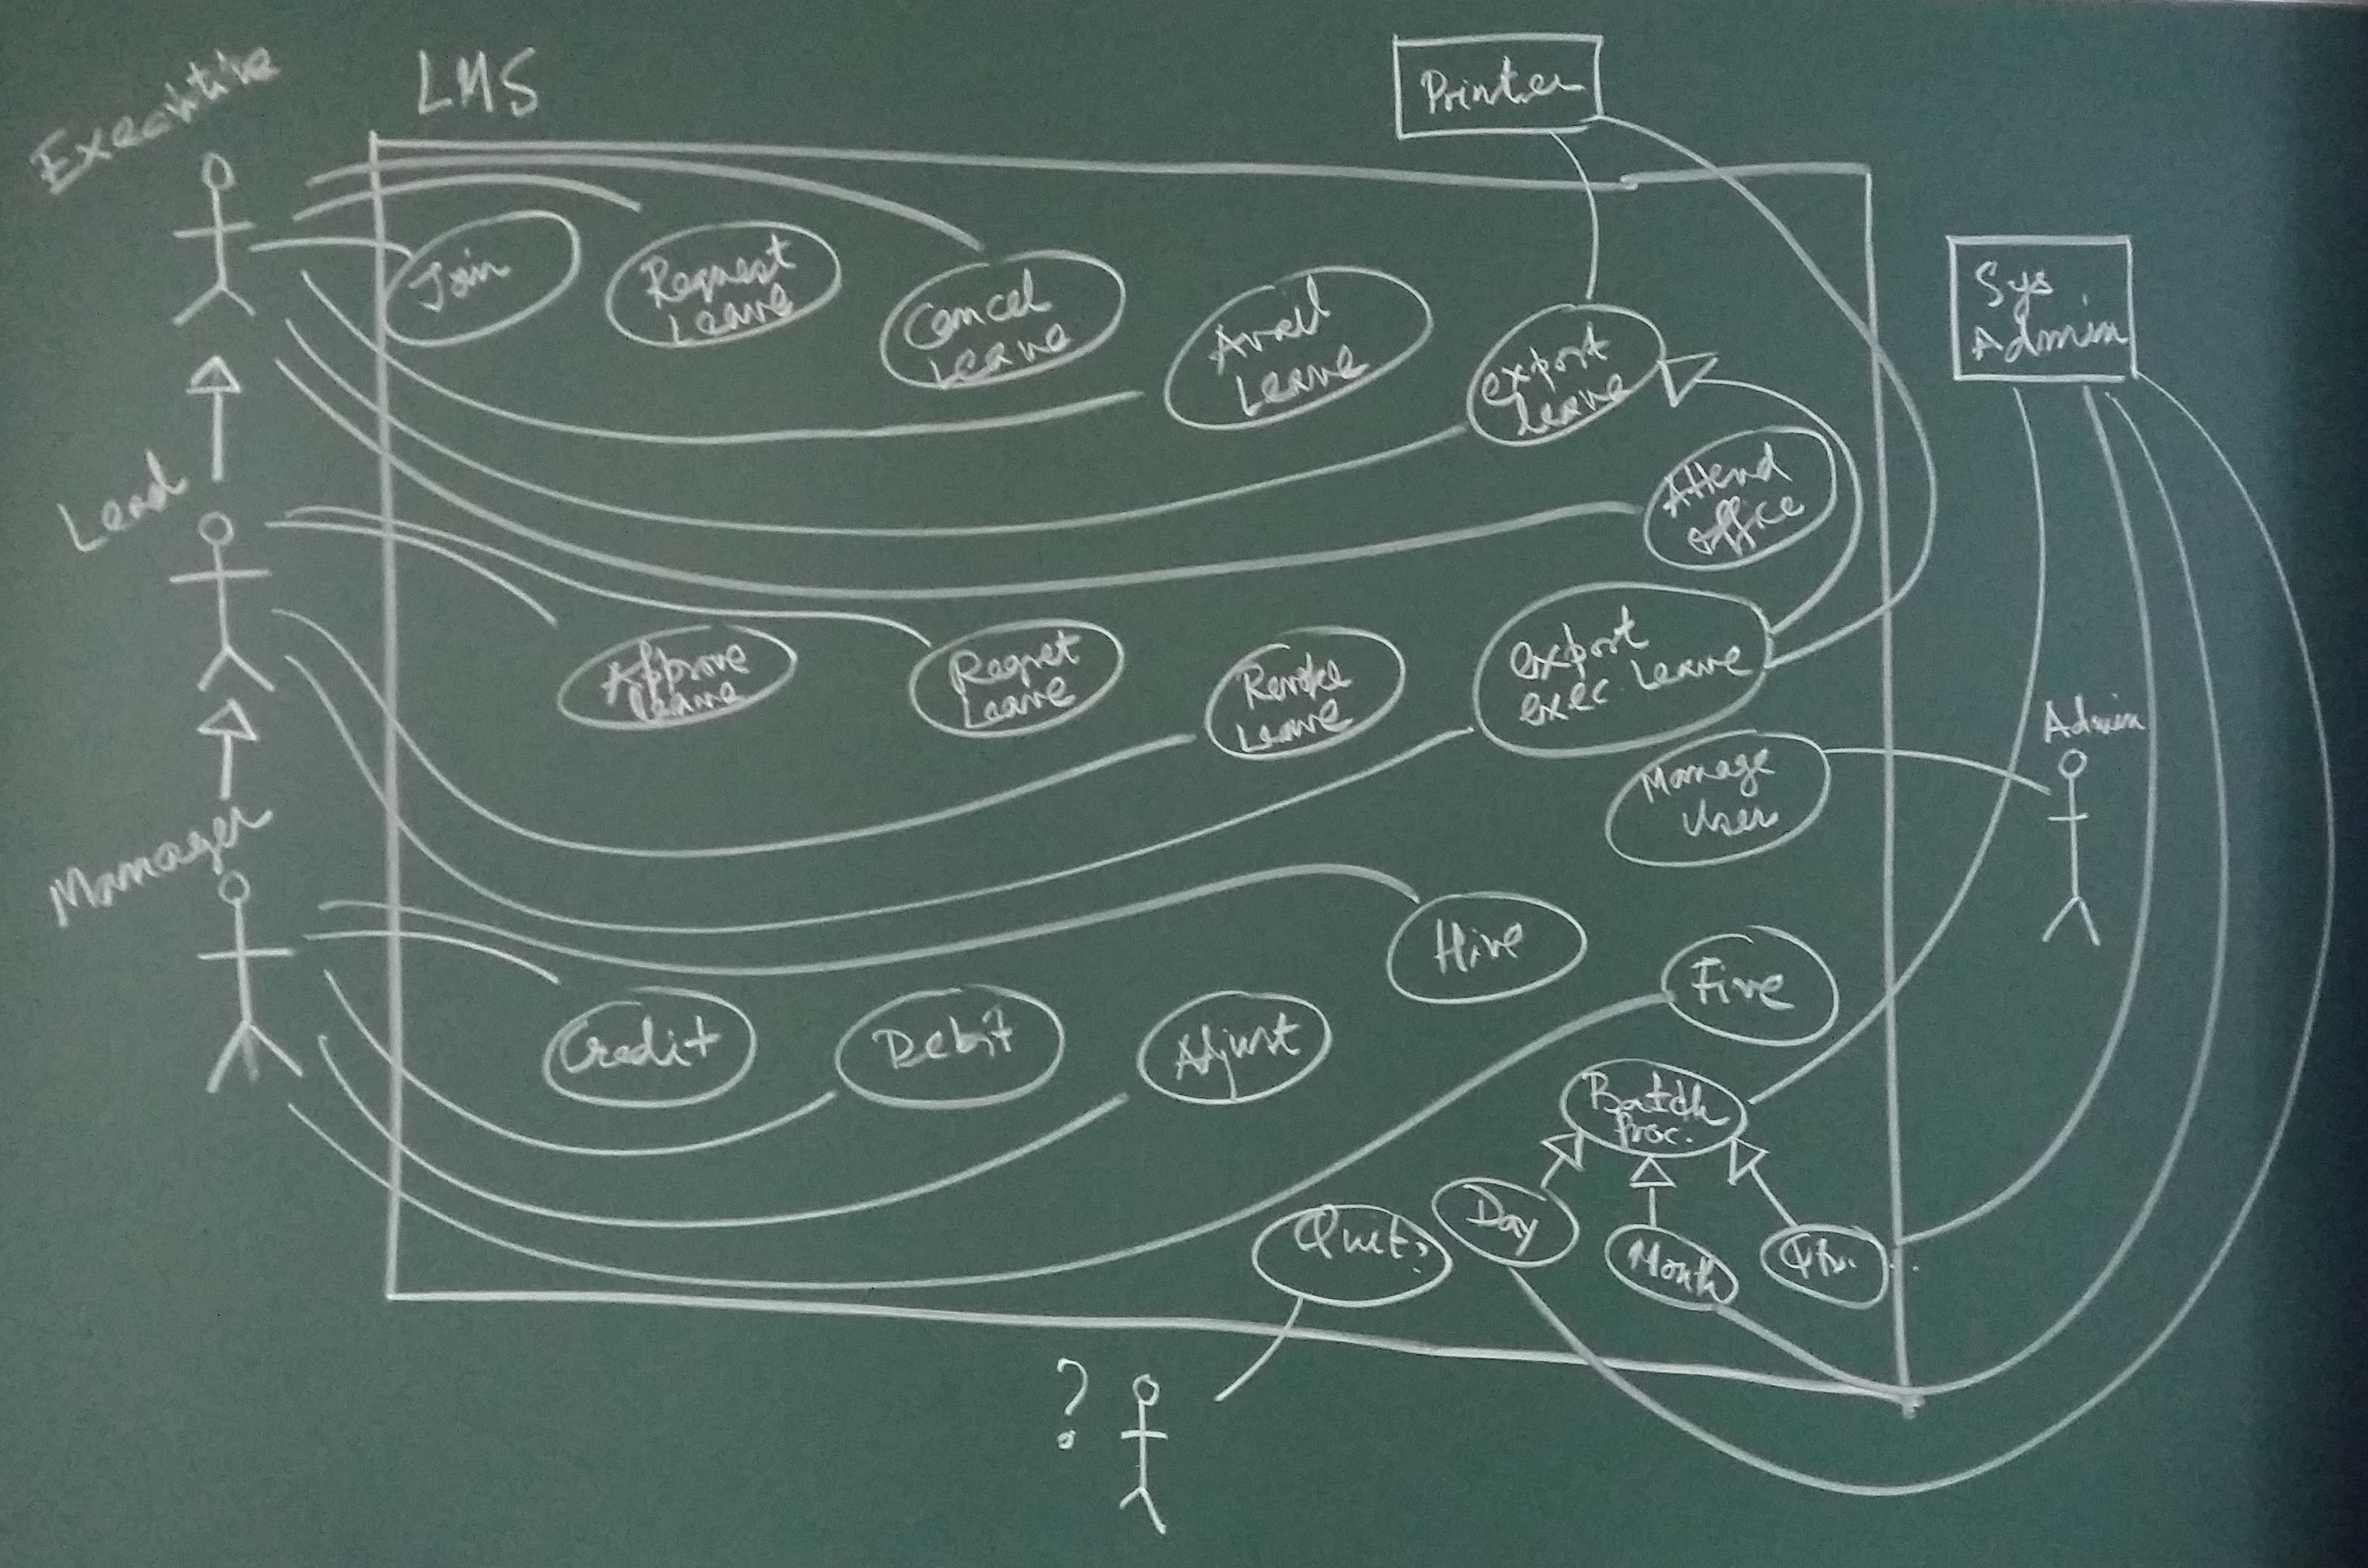
\includegraphics[width=12cm]{Images/Use-Case.jpg}
\caption{Use-Case Diagram of LMS
\label{fig:use-case}
}
\end{figure}

\newpage
\begin{figure}[ht]
\centering
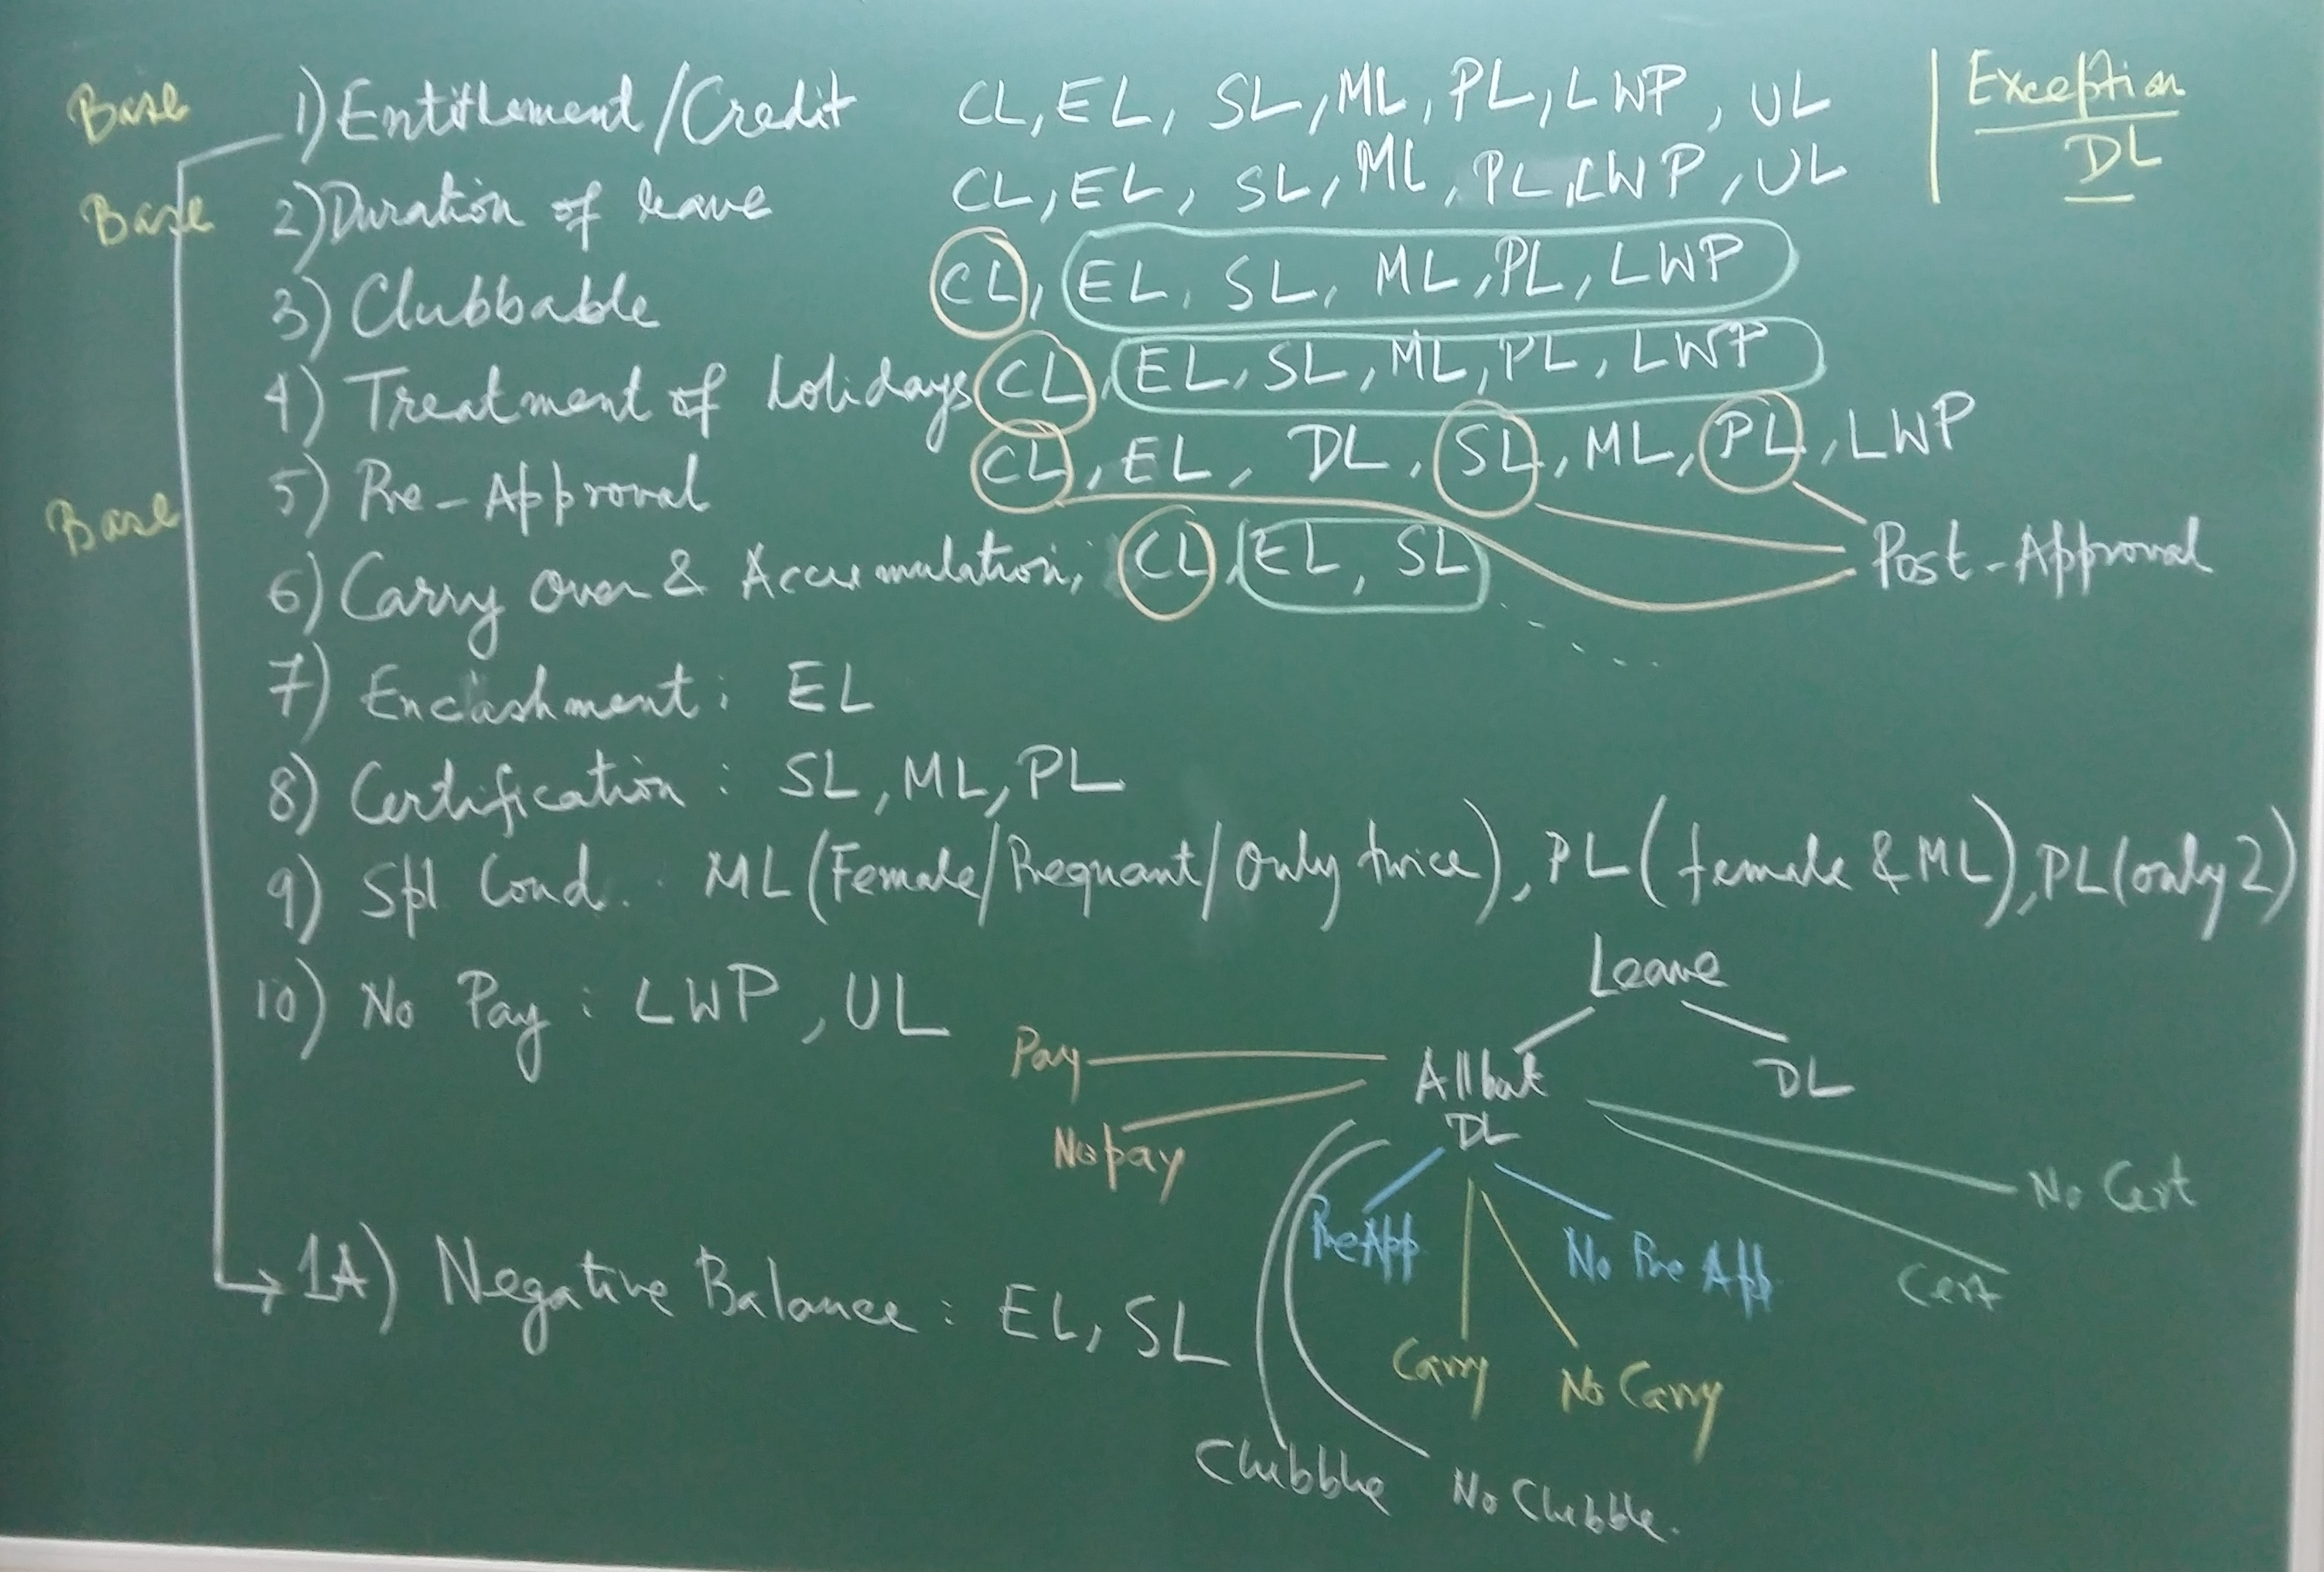
\includegraphics[width=12cm]{Images/Leave_Attributes.jpg}
\caption{Analysis of Leaves of LMS
\label{fig:use-case}
}
\end{figure}

\begin{center}

\begin{tabular}{|l|c|c|c|c|c|c|c|c|}\hline
\multicolumn{1}{|c|}{\bf Property} & 
\multicolumn{1}{c|}{\bf CL} &
\multicolumn{1}{c|}{\bf EL} &
\multicolumn{1}{c|}{\bf SL} &
\multicolumn{1}{c|}{\bf DL} &
\multicolumn{1}{c|}{\bf ML} &
\multicolumn{1}{c|}{\bf PL} &
\multicolumn{1}{c|}{\bf LWP} &
\multicolumn{1}{c|}{\bf UL} \\ \hline
{\em Entitlement} & Y & Y & Y & NA & Y$^a$ & Y & Y & N$^b$ \\ \hline
{\em Duration of Leave} & Y & Y & Y & NA & Y & Y & Y & N$^c$ \\ \hline
{\em Is Leave Clubbable?} & N & Y & Y & NA & Y & Y & Y & N \\ \hline
{\em Is Holiday exempt in Leave?} & Y & N & N & NA & N & N & N & N \\ \hline
{\em Must Leave be Pre-Approved?} & N & Y & N$^d$ & NA & Y & N$^e$ & Y & N \\ \hline
{\em Does Leave Carry-over \& Accumulate?} & N & Y & Y & NA & N & N & N & N \\ \hline
{\em Can Leave by En-cashed?} & N & Y & N & NA & N & N & N & N \\ \hline
{\em Does Leave need Certification?} & N & N & Y & NA & Y & Y & N & N \\ \hline
{\em Is Leave paid?} & Y & Y & Y & NA & Y & Y & N & N \\ \hline \hline
\multicolumn{9}{l}{$^a$: Only for female, when pregnant, twice in career} \\ 
\multicolumn{9}{l}{$^b$: Deemed entitlement for a week before actions start} \\ 
\multicolumn{9}{l}{$^c$: Allowed for up to a 7 days} \\ 
\multicolumn{9}{l}{$^d$: Exception condition for sickness} \\ 
\multicolumn{9}{l}{$^e$: Exception condition for parenthood} \\ 
\end{tabular}

\end{center}

\newpage
\begin{figure}[ht]
\centering
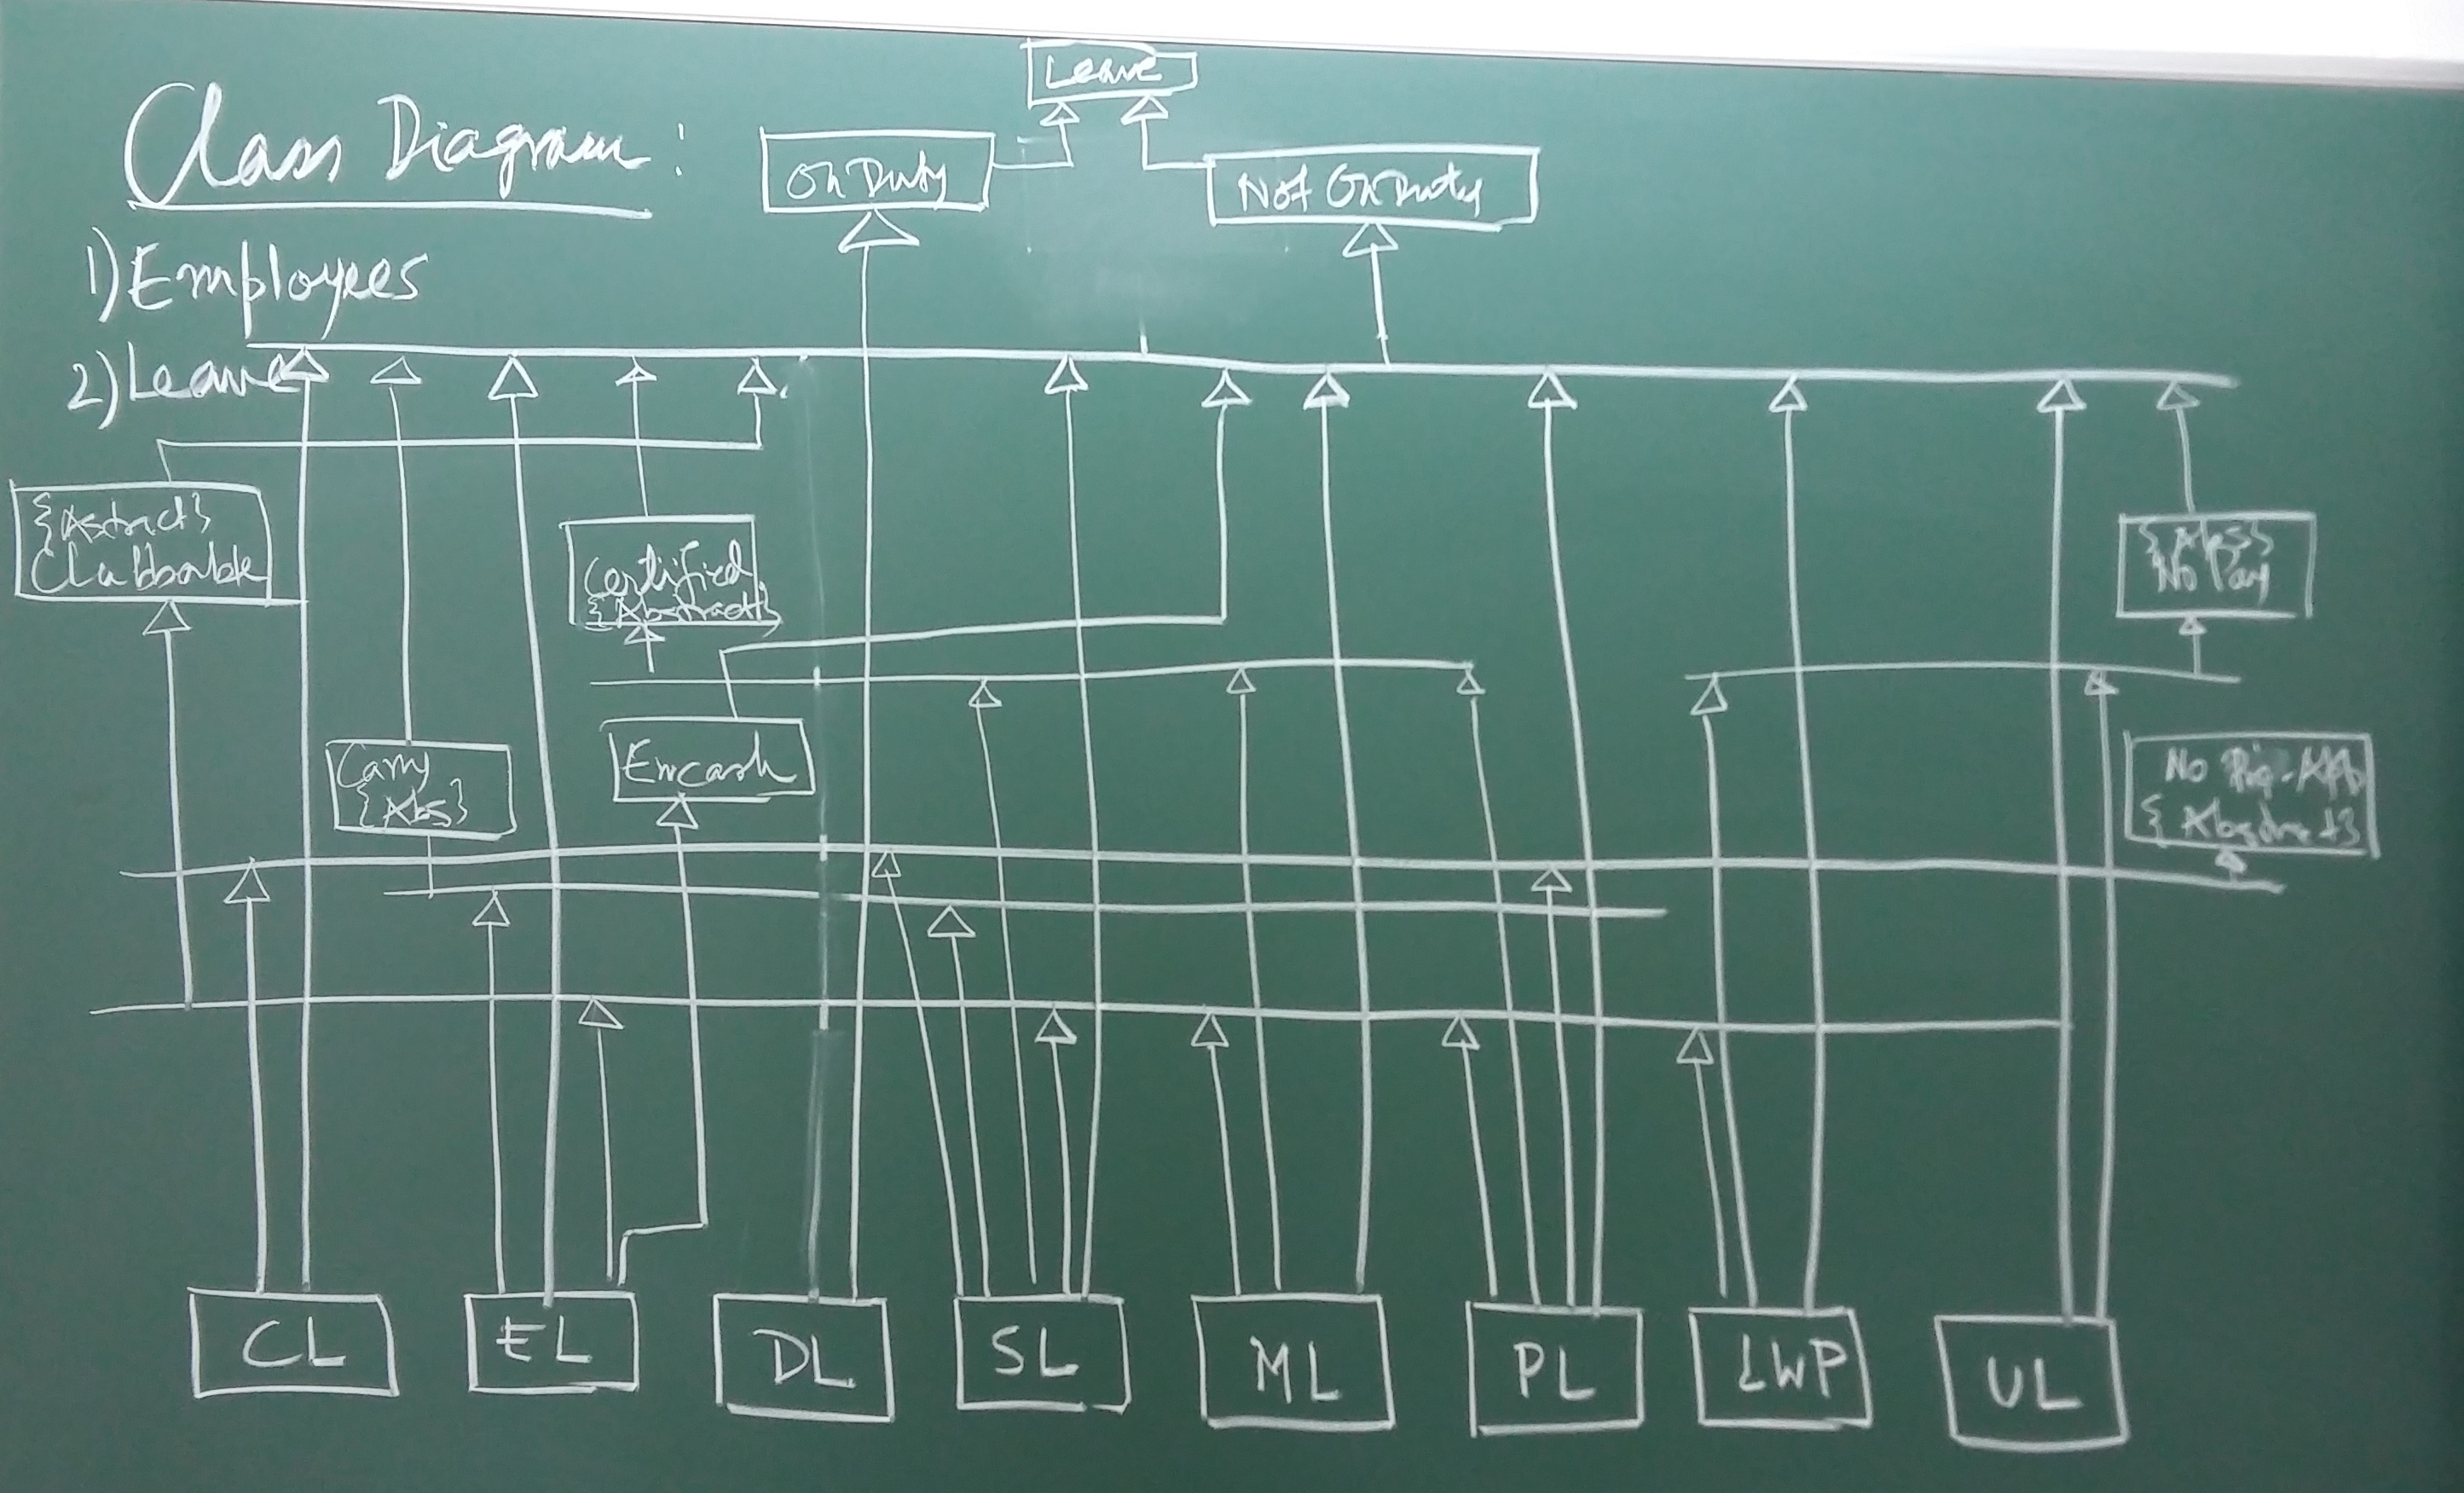
\includegraphics[width=12cm]{Images/Class_1.jpg}
\caption{Class Diagram (Leave) of LMS
\label{fig:use-case}
}
\end{figure}

\begin{figure}[ht]
\centering
\begin{tabular}{ll}
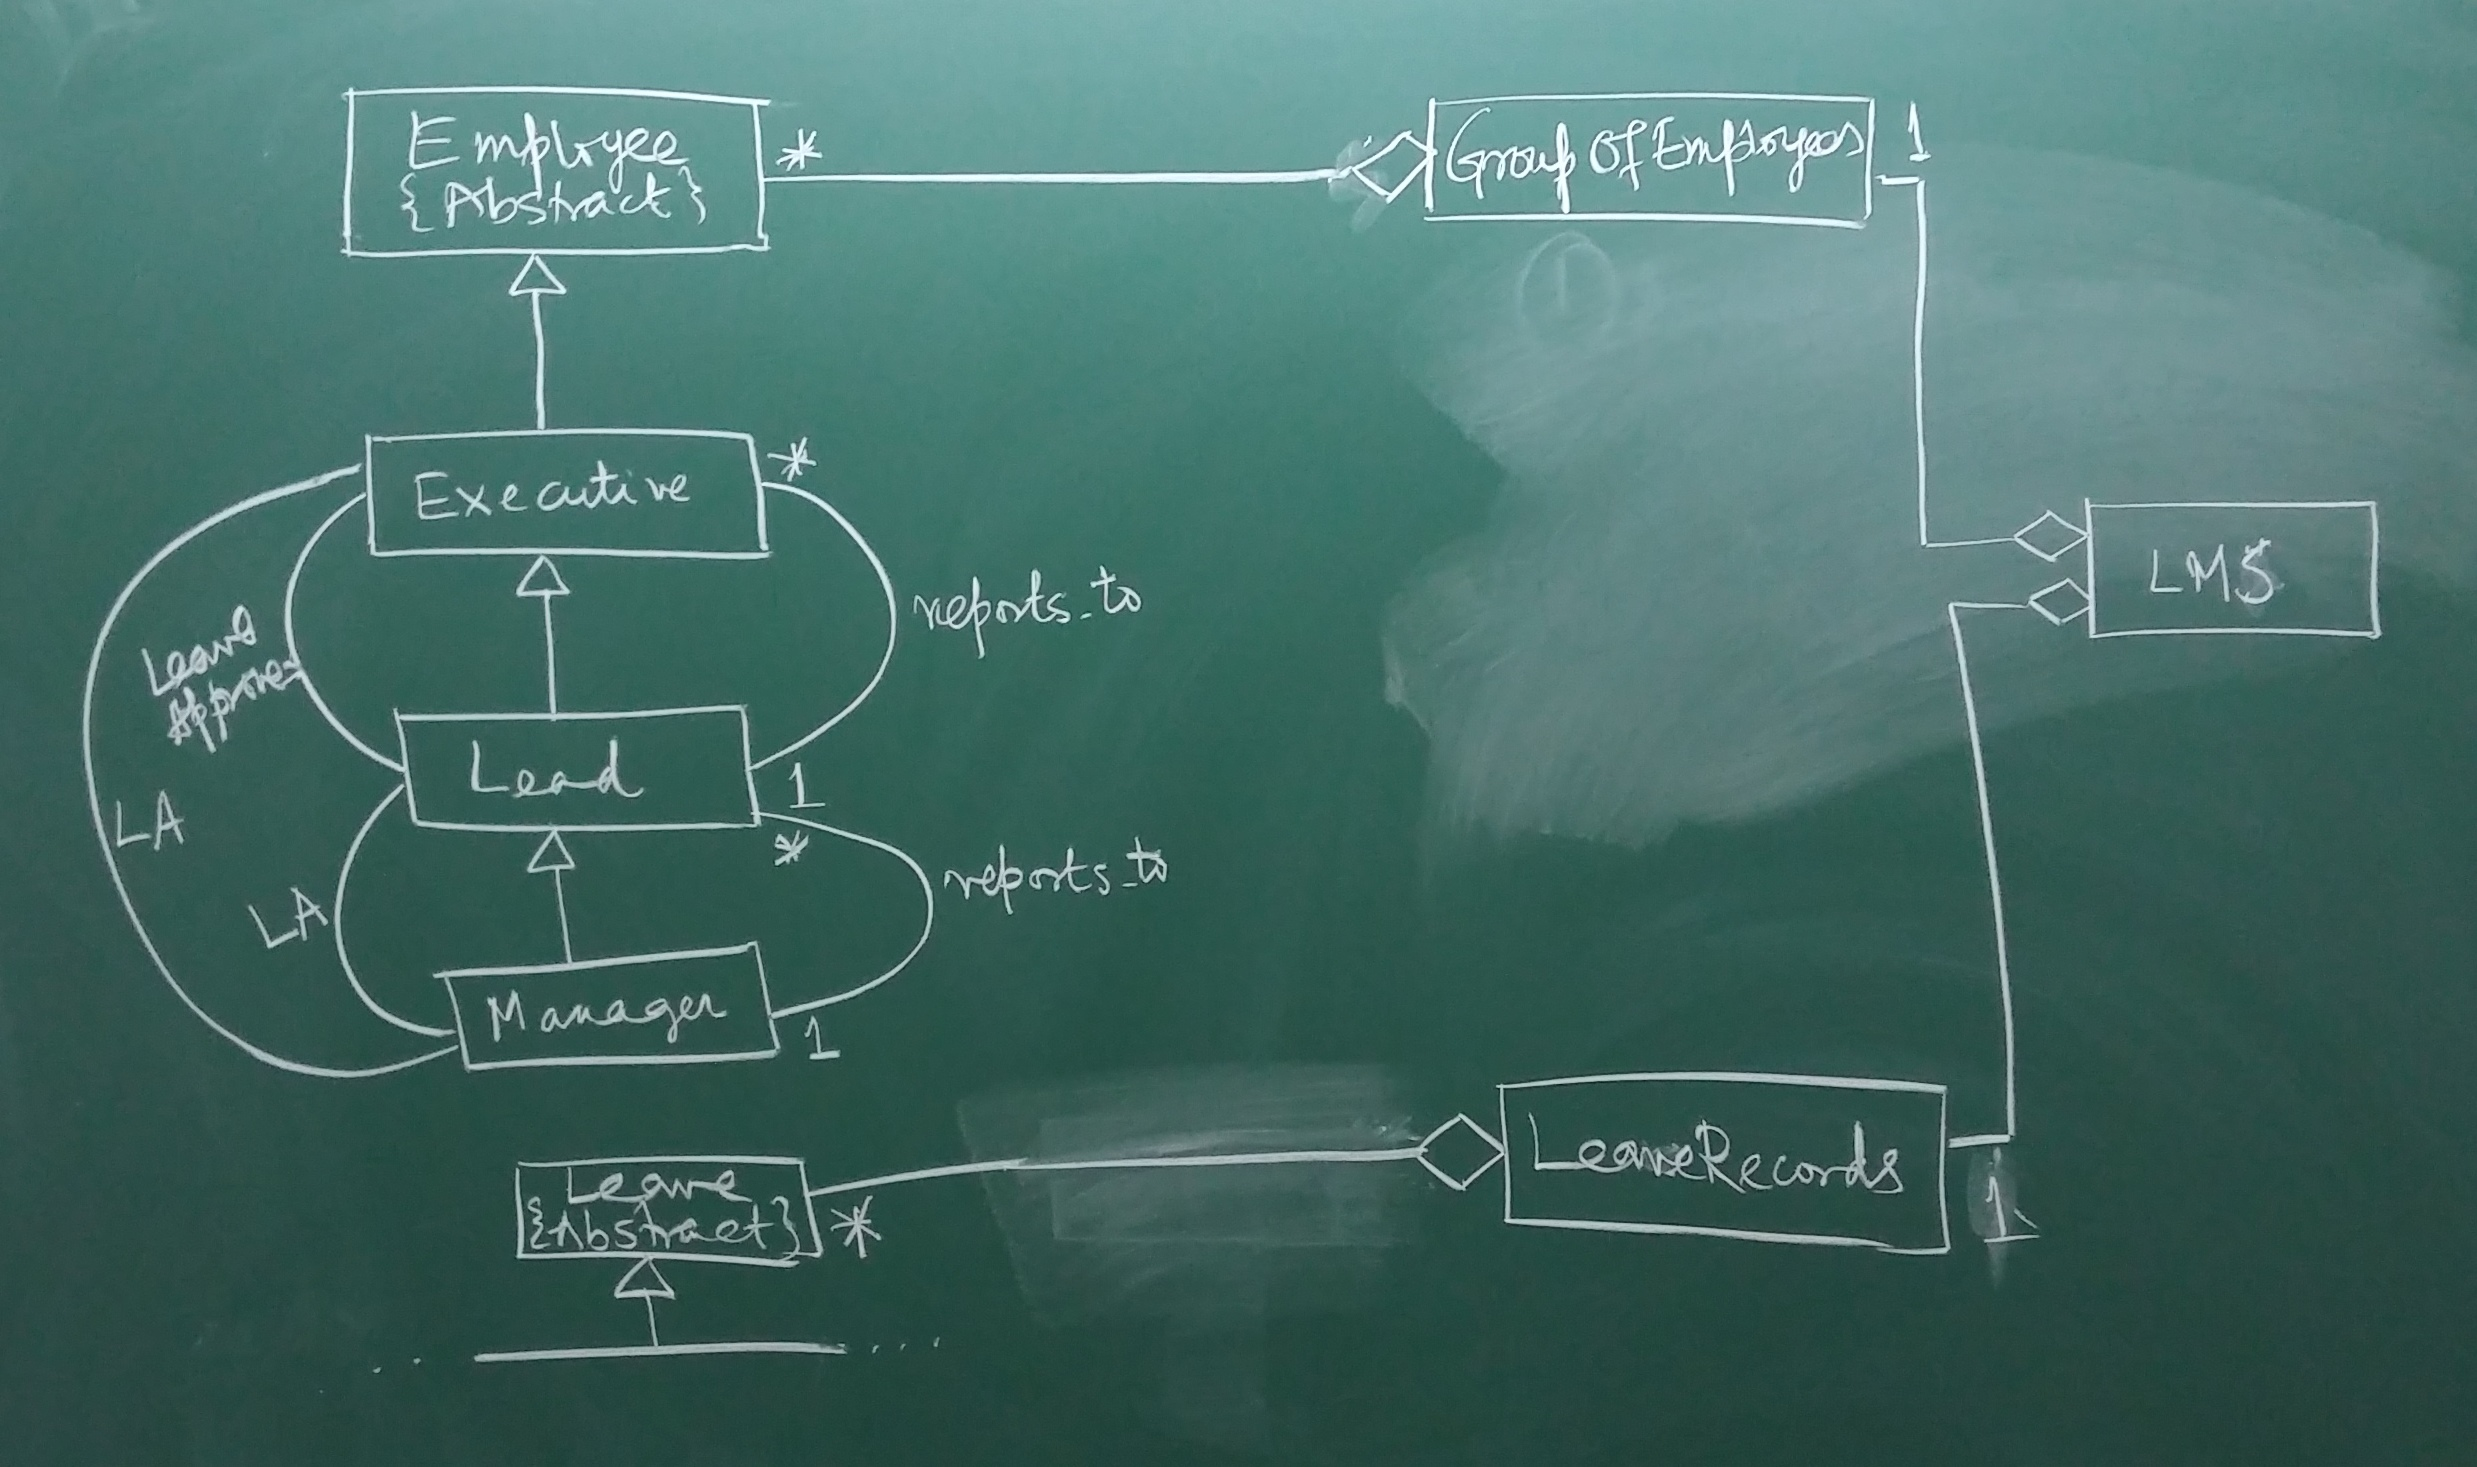
\includegraphics[width=12cm]{Images/Class_2.jpg} &
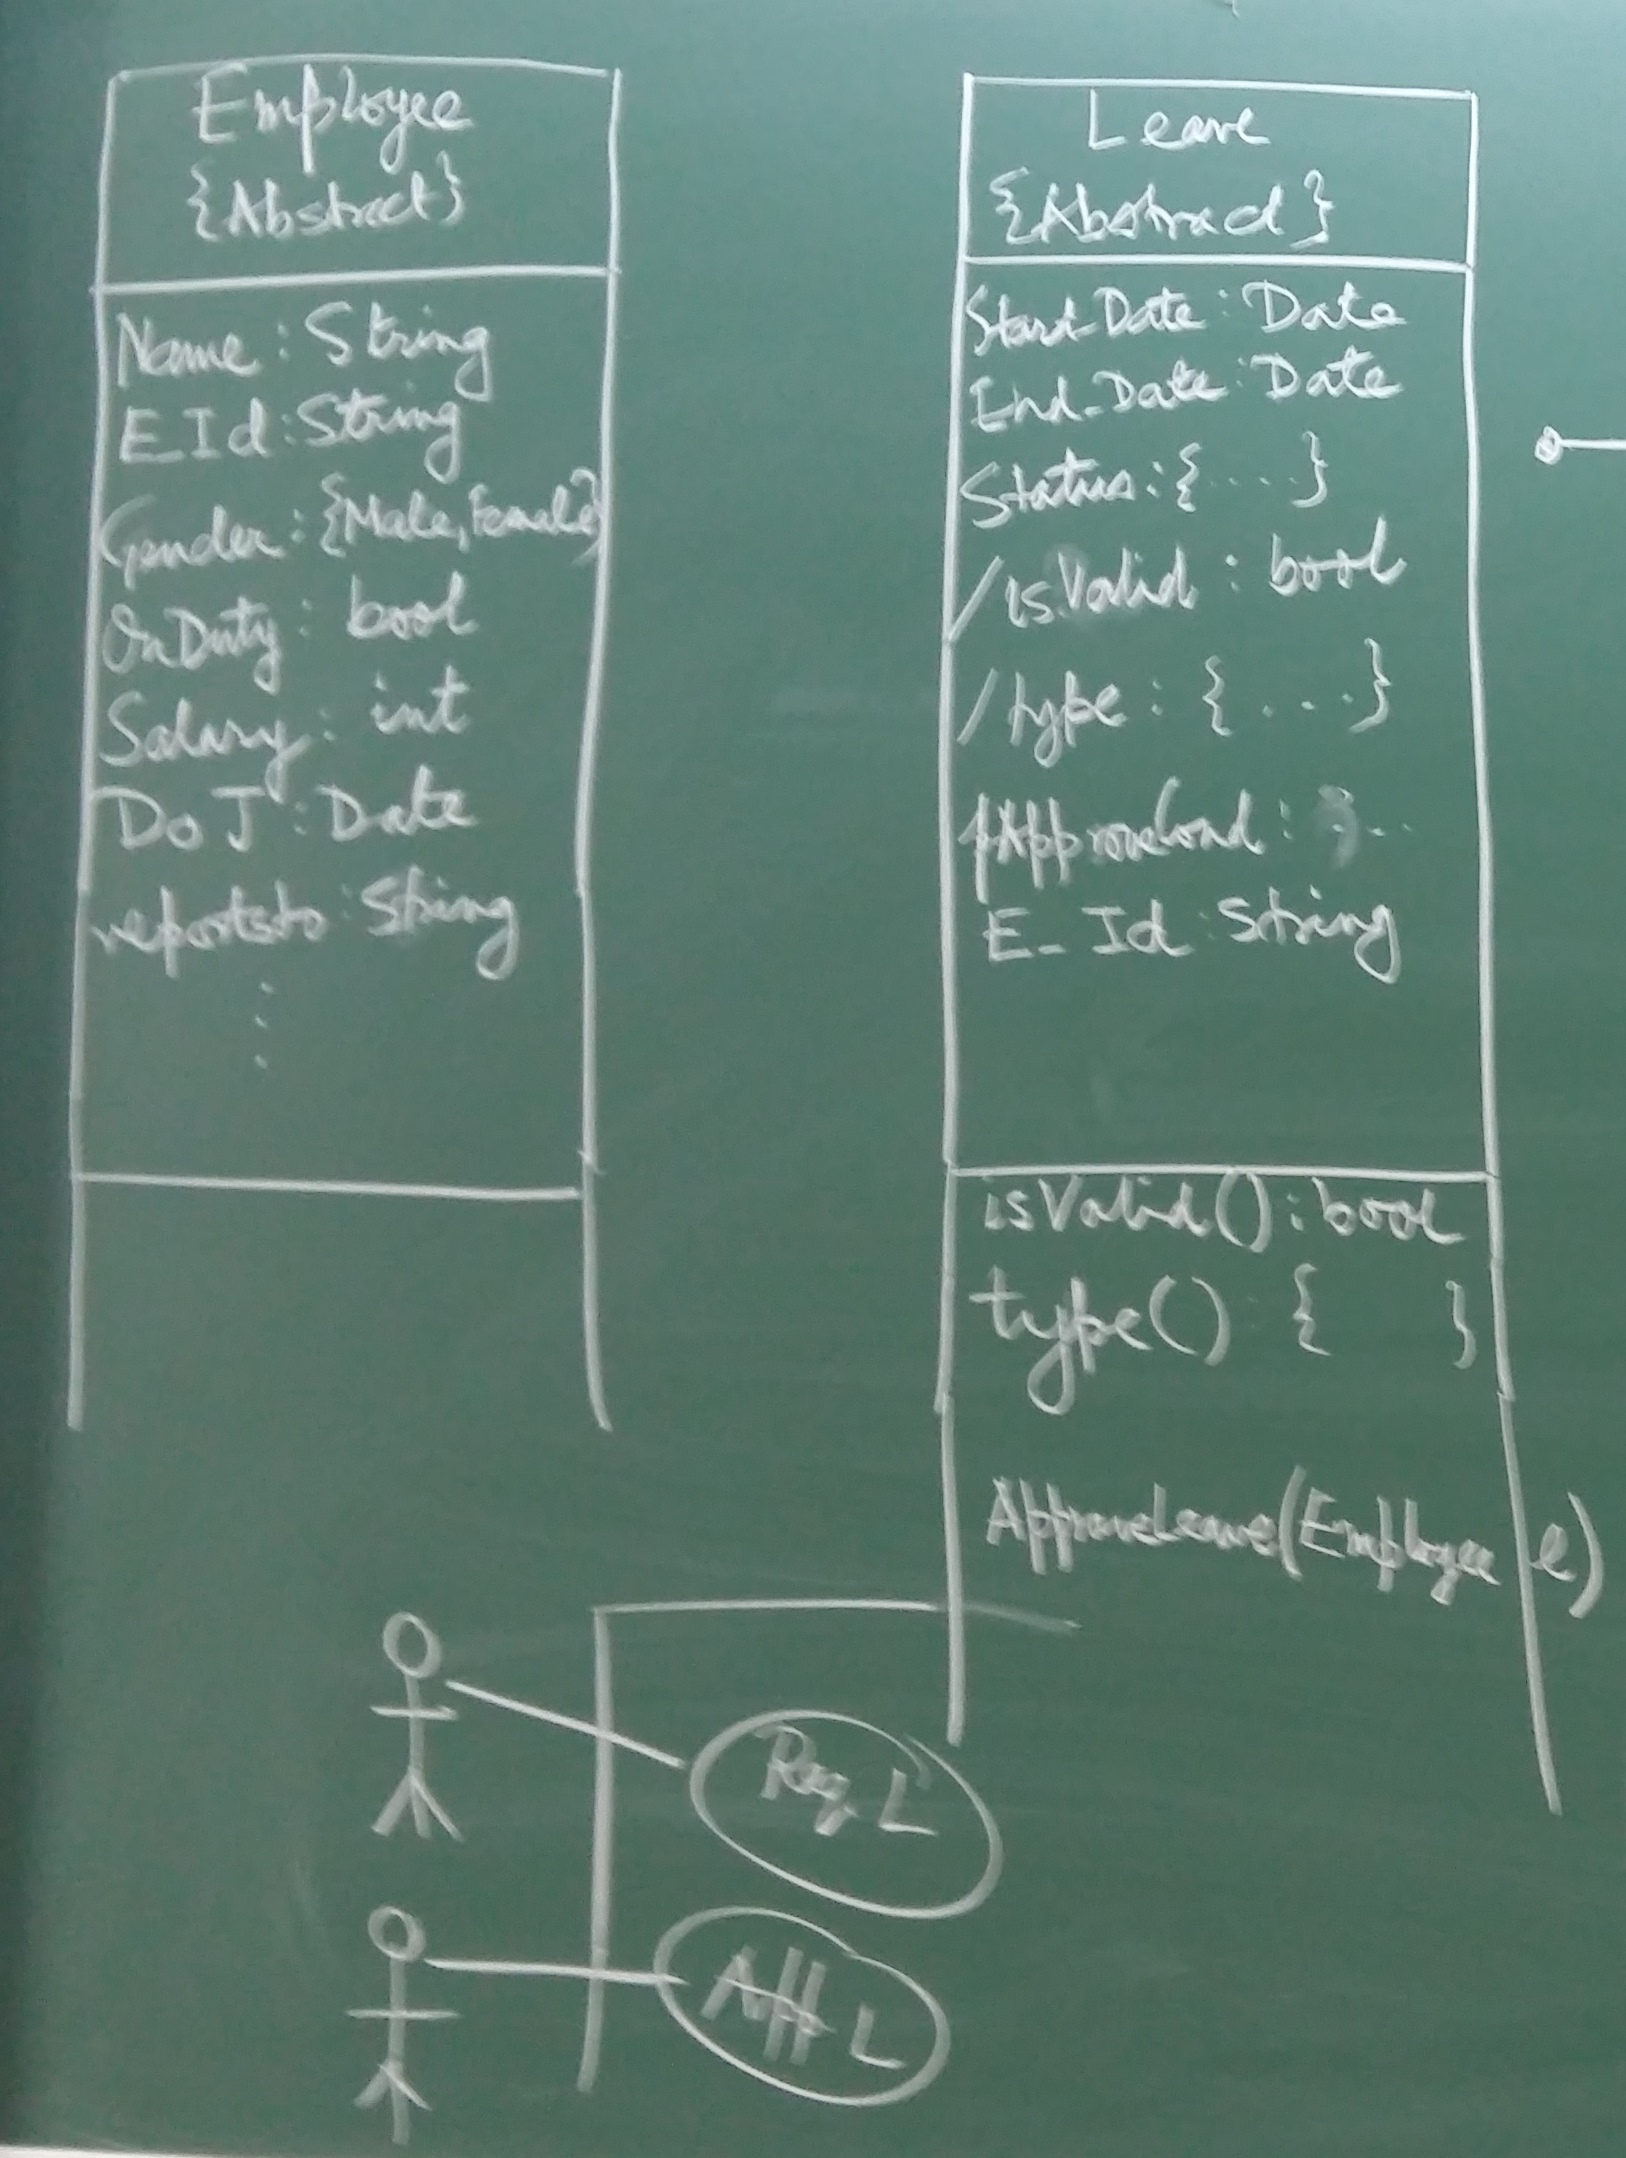
\includegraphics[width=6cm]{Images/Class_3.jpg}
\end{tabular}
\caption{Class Diagrams and Associations of LMS
\label{fig:use-case}
}
\end{figure}

\begin{figure}[!ht]
\centering
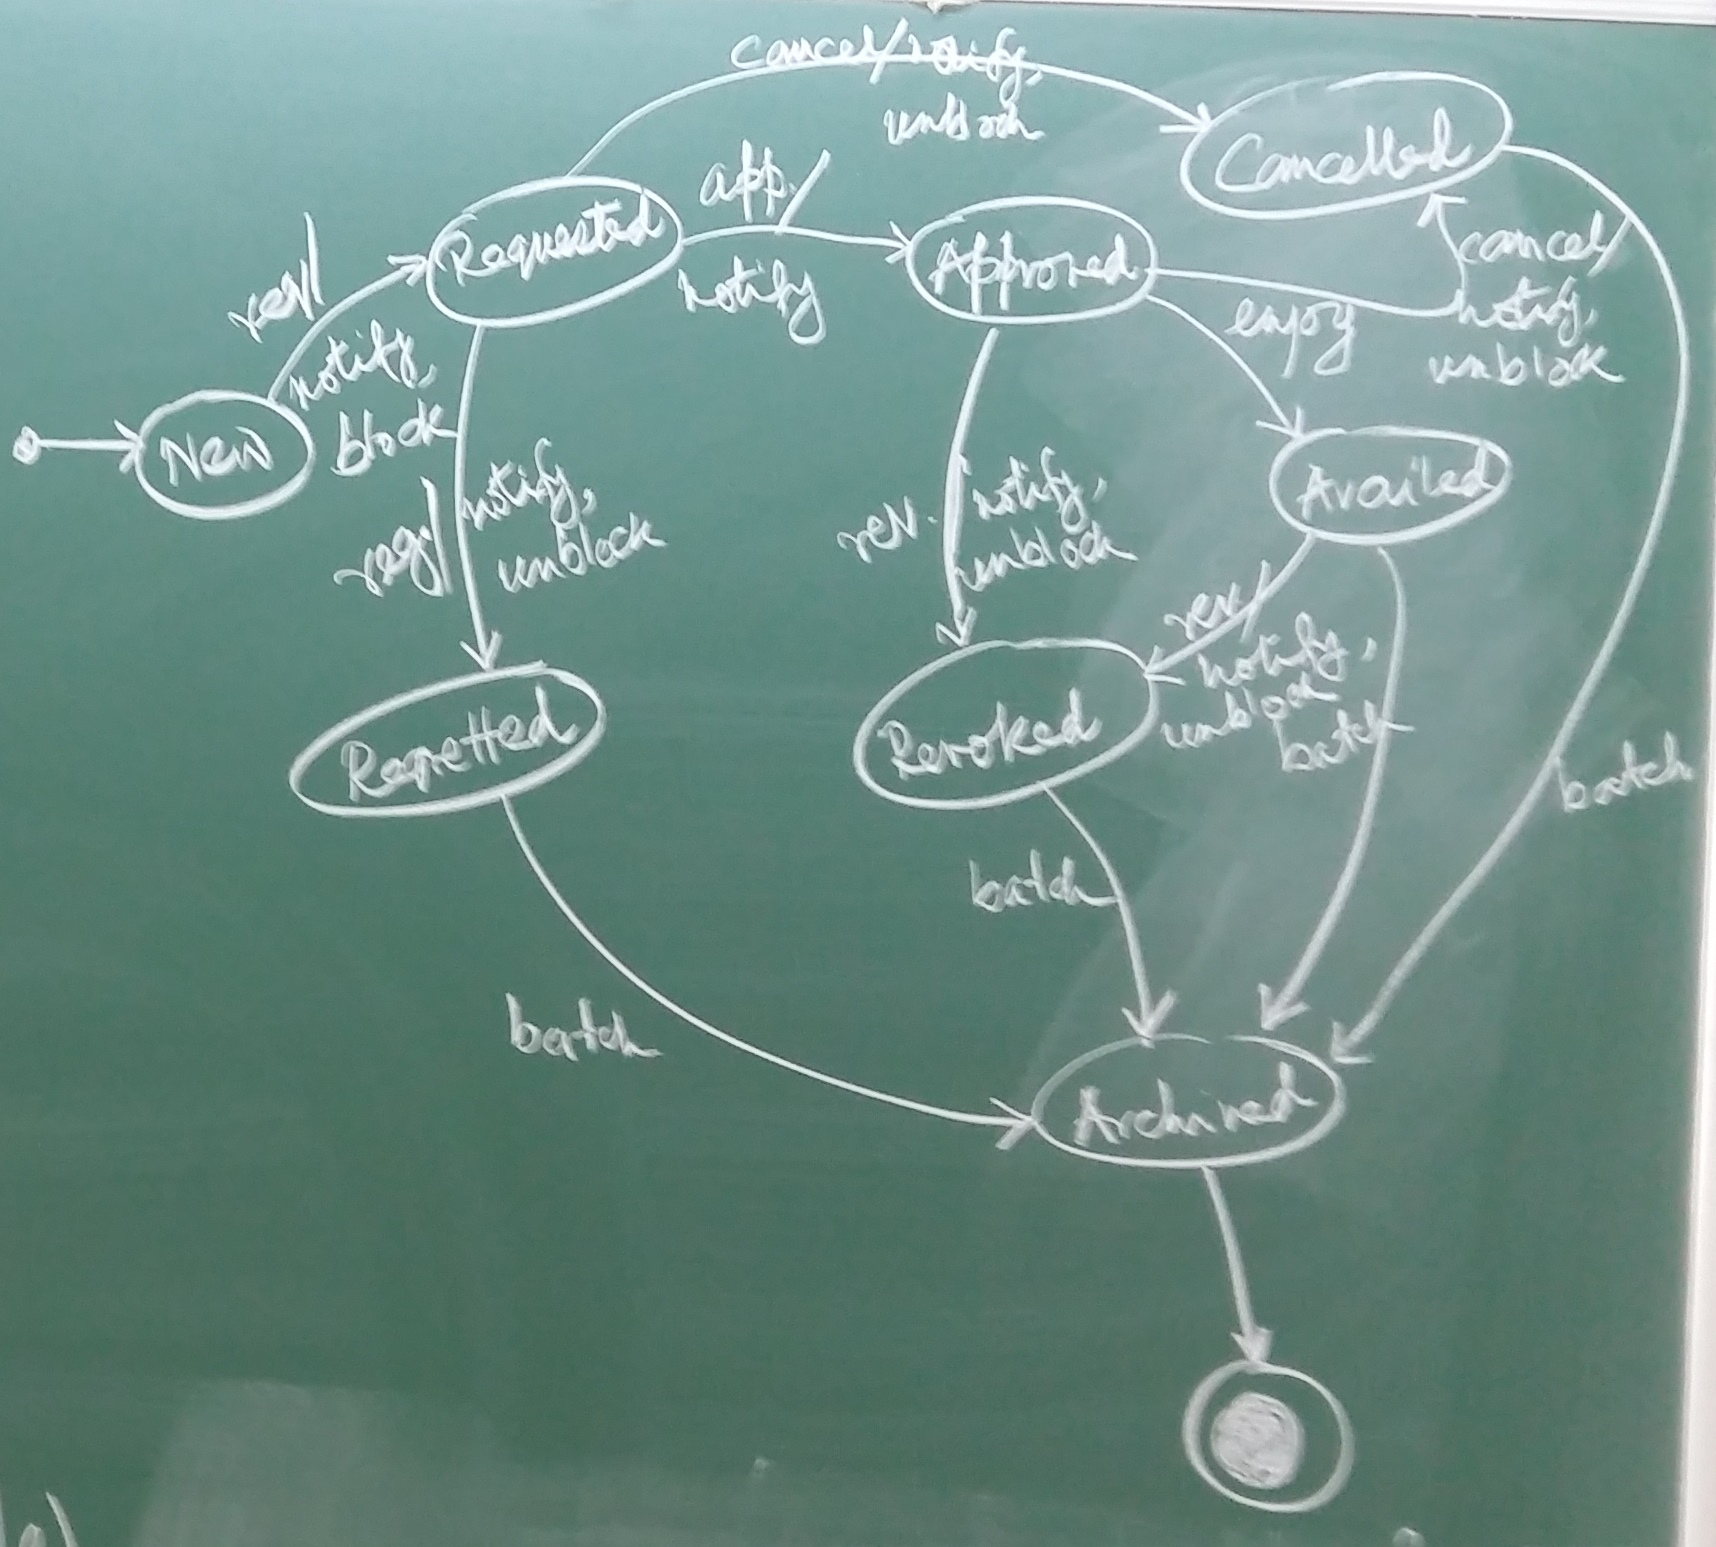
\includegraphics[width=8cm]{Images/StateChart.jpg}
\caption{StateChart Diagram of LMS (Leave)
\label{fig:use-case}
}
\end{figure}

\begin{figure}[!ht]
\centering
\begin{tabular}{ll}
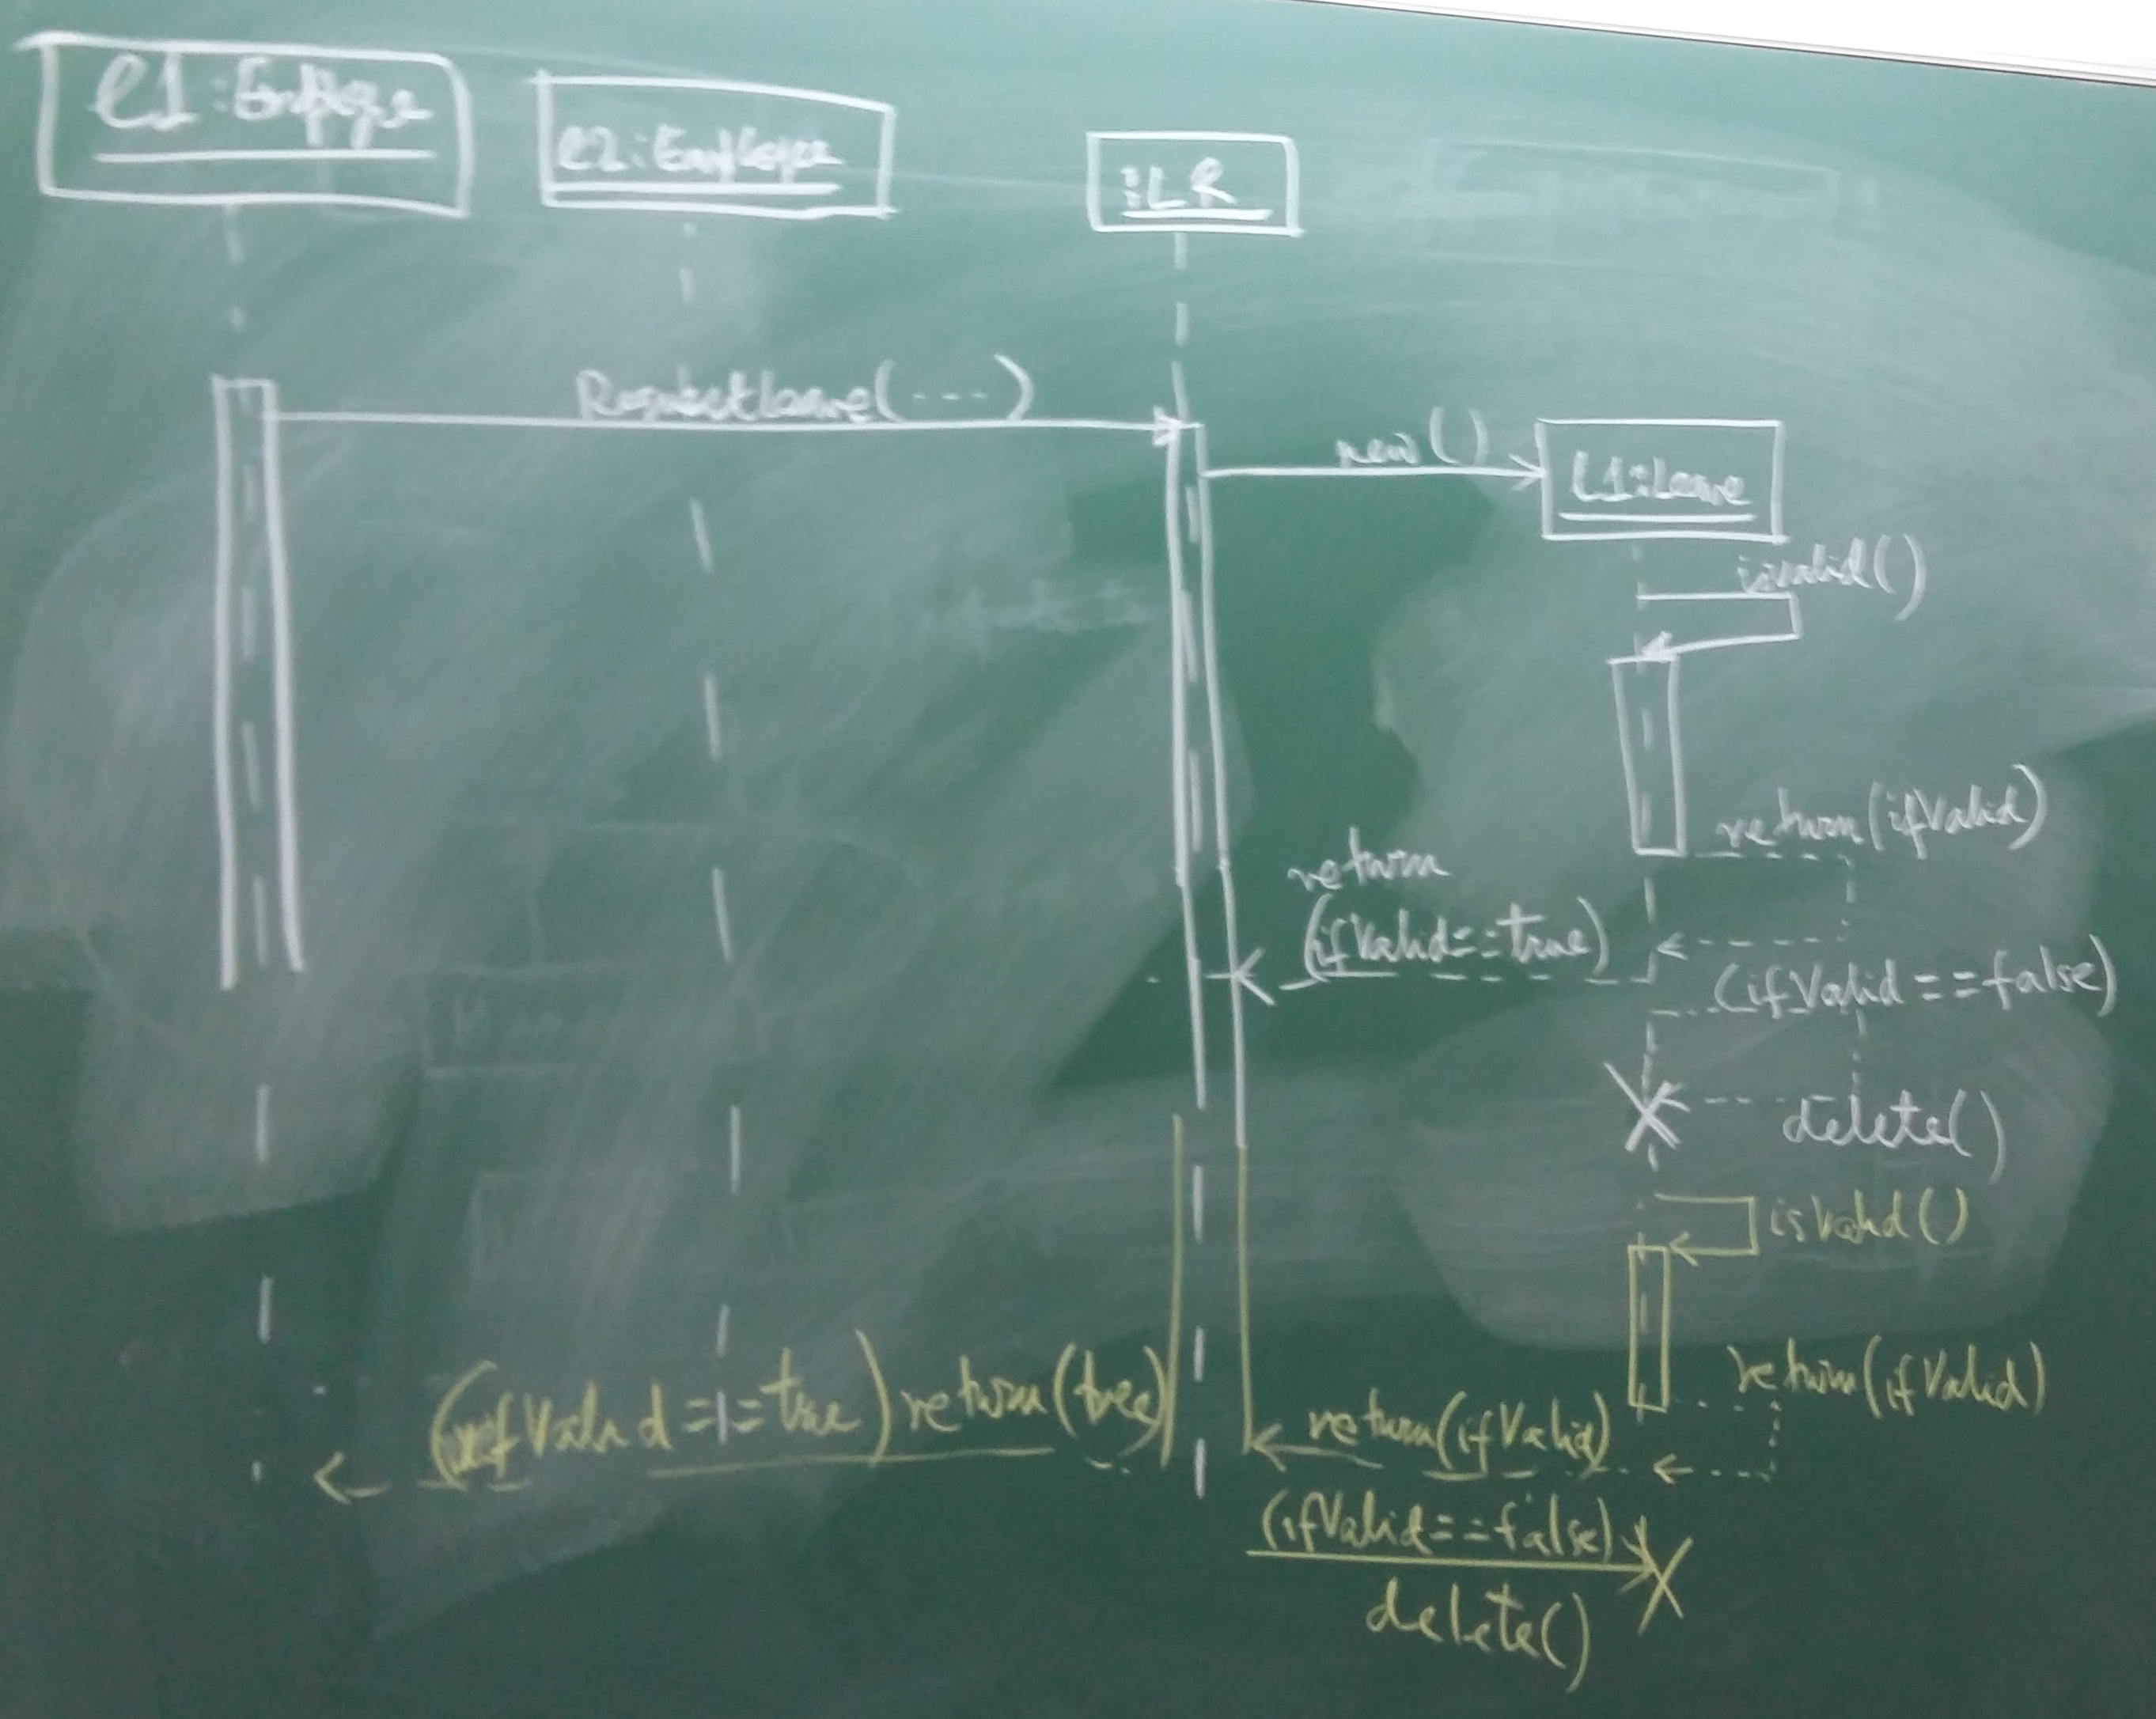
\includegraphics[width=9cm]{Images/Sequence_1.jpg} &
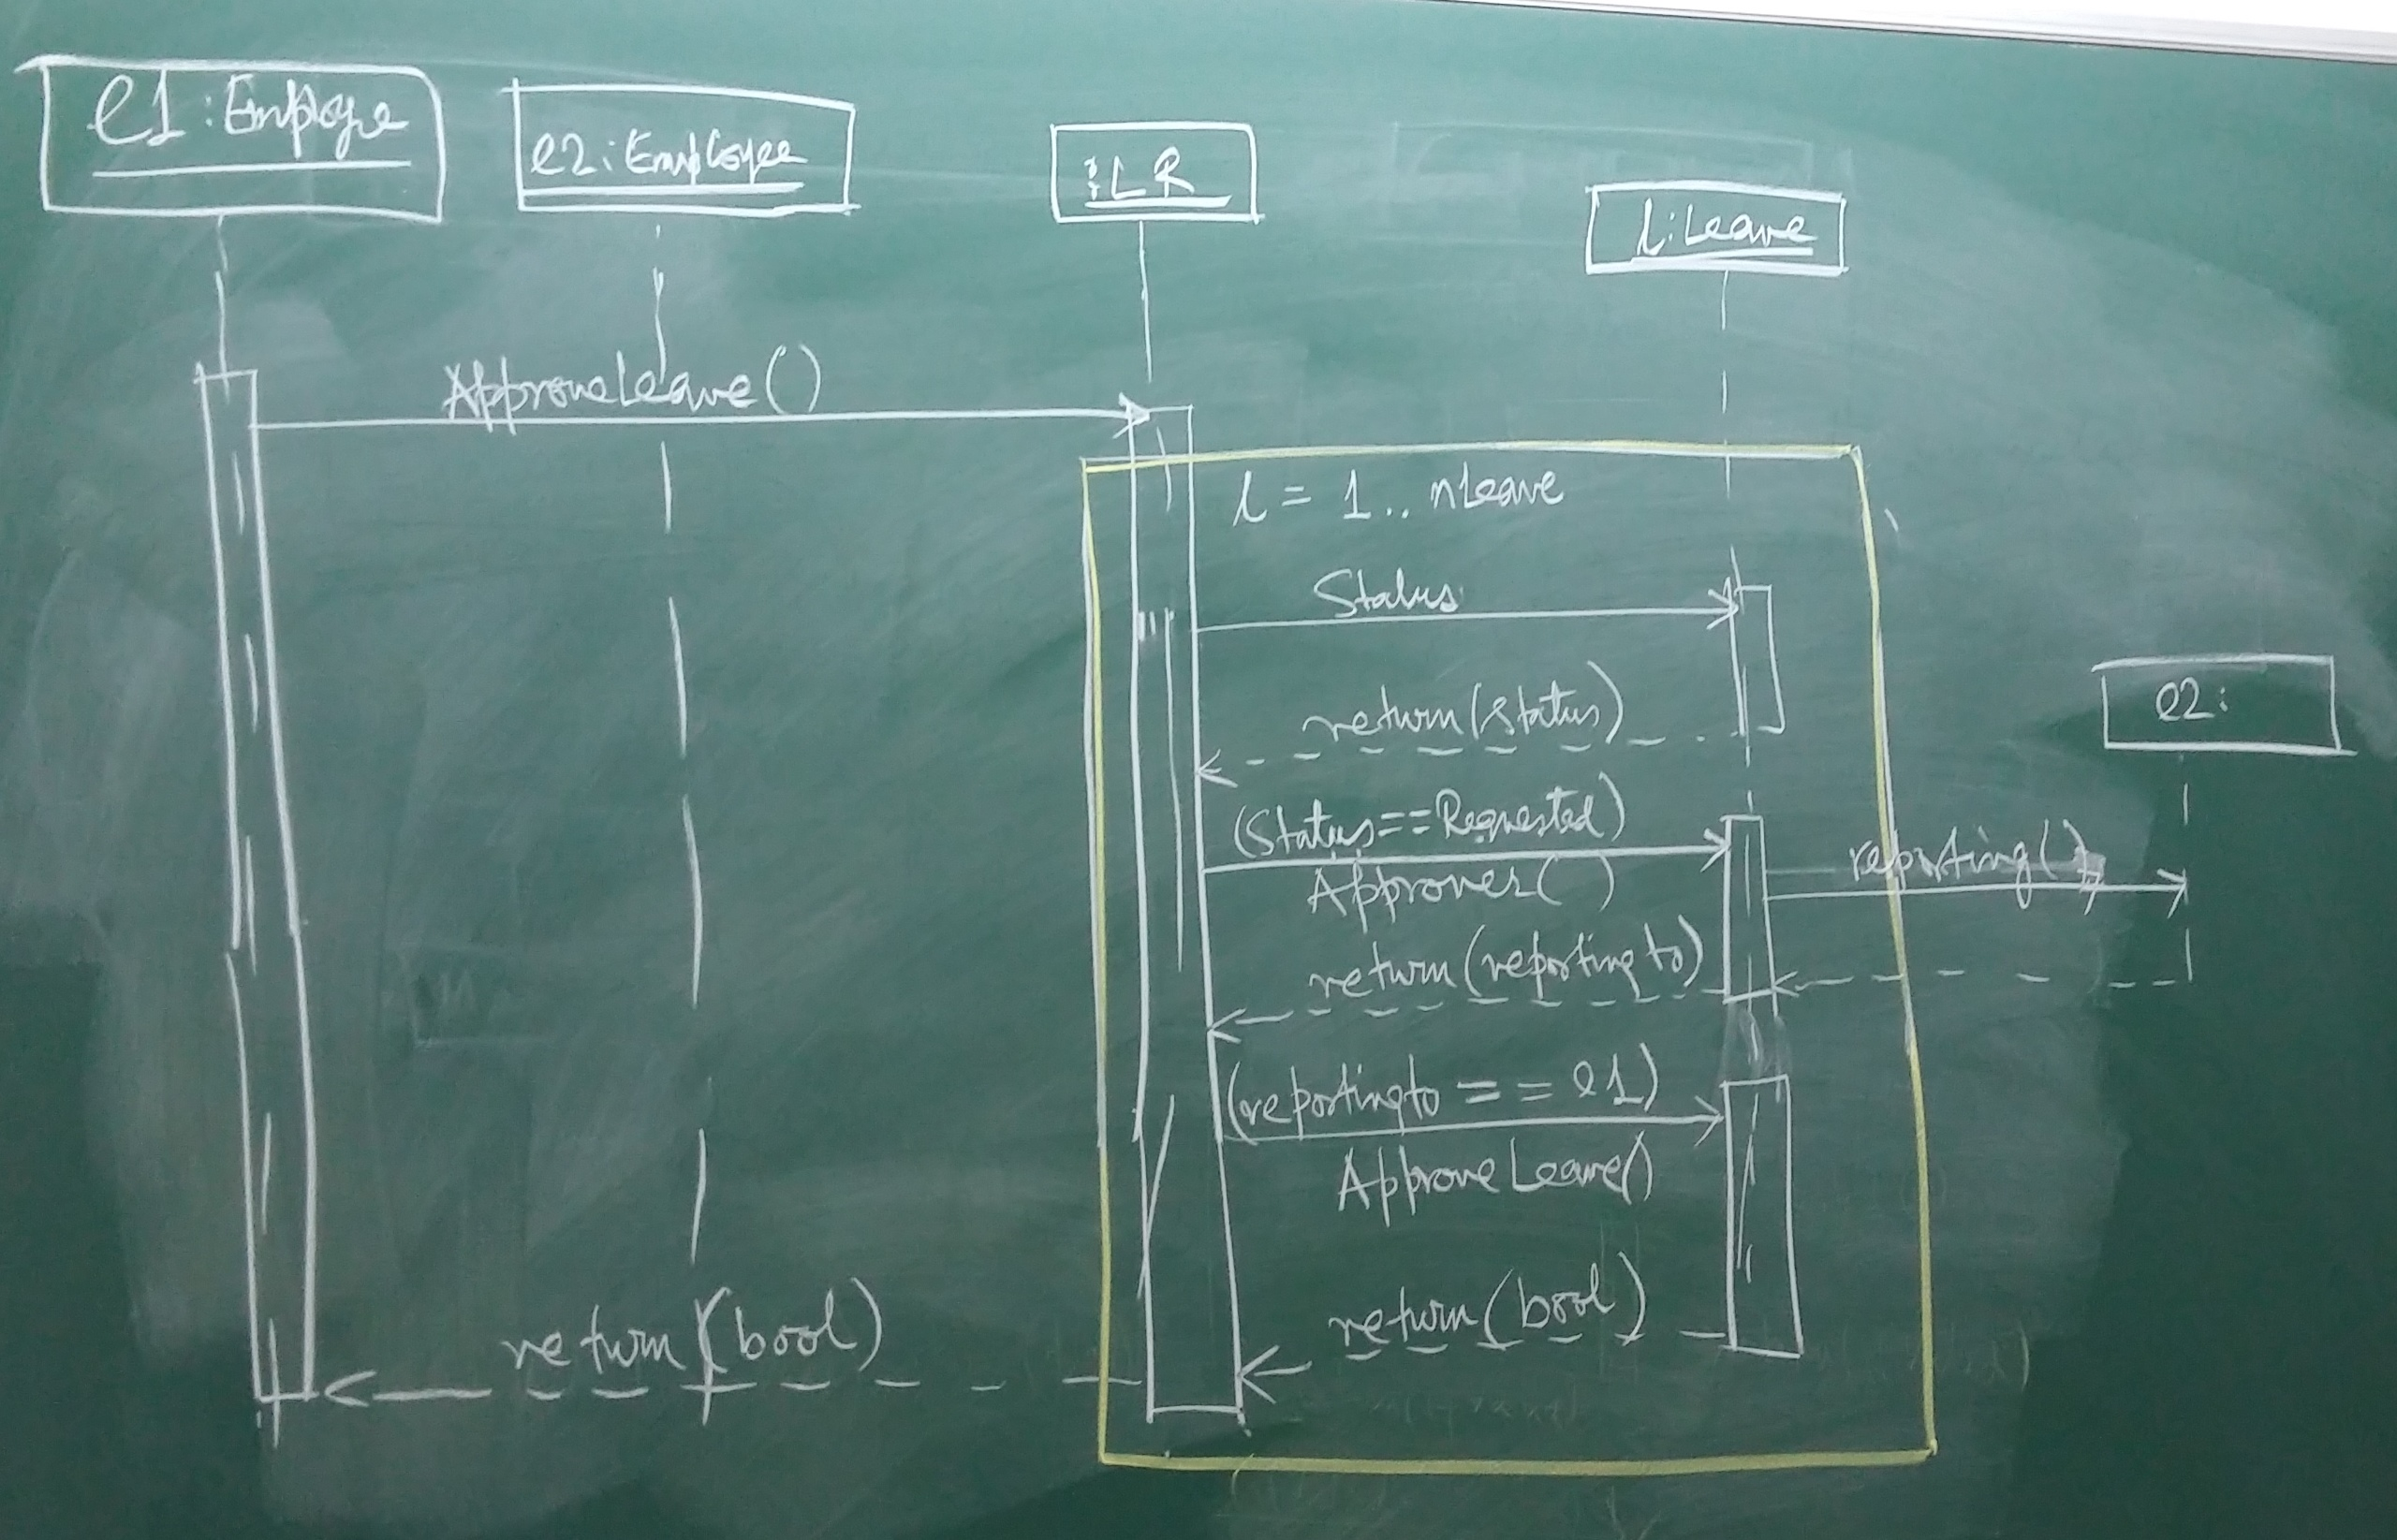
\includegraphics[width=9cm]{Images/Sequence_2.jpg}
\end{tabular}
\caption{Sequence Diagrams of LMS
\label{fig:use-case}
}
\end{figure}

\vspace*{10cm}
\newpage

\section*{Testplan}
%\begin{table} [!ht]
%\caption{Testplan of LMS
%\label{fig:use-case}
%}
\begin{footnotesize}
\begin{center}
\begin{tabular}{|l||l|l|l|l|l|l|l|p{6cm}|} \hline
\multicolumn{9}{|c|}{\bf Leave Quota} \\ \hline
Test & CL & EL & DL & SL & ML & PL & LWP & Remarks \\ \hline \hline
Credit 				&&&X&&&&& Checks if leave is rightly credited \\ \hline
Carry Forward 		&&&X&&&&& Checks if leave is rightly carried forward to next period \\ \hline
Brought Over		&&&X&&&&& Checks if leave is rightly brought over from previous period \\ \hline
Encashment			&X&&X&X&X&X&X& Checks if leave is rightly transferred for encashment \\ \hline
\multicolumn{9}{|c|}{\bf Leave Period} \\ \hline
Test & CL & EL & DL & SL & ML & PL & LWP & Remarks \\ \hline \hline
Duration			&&&&&&&& Checks if the leave is within permissible number of days\\ \hline
Holiday Mix			&&&&&&&& Checks if the leave mixes right with holidays - before, after, during, etc\\ \hline
Leave-Leave Mix		&&&&&&&& Checks if the leave mixes right with other leaves \\ \hline
\multicolumn{9}{|c|}{\bf Leave Financial} \\ \hline
Test & CL & EL & DL & SL & ML & PL & LWP & Remarks \\ \hline \hline
Encashment Credit	&X&&X&X&X&X&X& Checks if leave is rightly encashed to salary \\ \hline
Salary Deduction	&X&X&X&X&X&X&& Checks if salary is rightly deducted / held back for exceeding leave quota \\ \hline
\multicolumn{9}{|c|}{\bf Leave Conditions} \\ \hline
Test & CL & EL & DL & SL & ML & PL & LWP & Remarks \\ \hline \hline
Pre-Approval		&&&&&&&& Checks if a leave is usually pre-approved\\ \hline
Post-Approval		&&X&&&X&X&X& Checks if a leave is post-approved under special circumstances\\ \hline
Medical				&X&X&X&&&X&& Checks the medical conditions and certificates for leave \\ \hline
Maternity			&X&X&X&X&&&& Checks the maternity conditions and certificates for leave \\ \hline
Parental			&X&X&X&X&&&X& Checks the parental conditions and certificates for leave \\ \hline
Exigency			&X&X&X&X&X&X&& Checks the exigency conditions and documents for leave \\ \hline
\end{tabular}
\end{center}
\end{footnotesize}
%\end{table}

\end{document}
